%  template.tex for Biometrics papers
%
%  This file provides a template for Biometrics authors.  Use this
%  template as the starting point for creating your manuscript document.
%  See the file biomsample.tex for an example of a full-blown manuscript.

%  ALWAYS USE THE referee OPTION WITH PAPERS SUBMITTED TO BIOMETRICS!!!
%  You can see what your paper would look like typeset by removing
%  the referee option.  Because the typeset version will be in two
%  columns, however, some of your equations may be too long. DO NOT
%  use the \longequation option discussed in the user guide!!!  This option
%  is reserved ONLY for equations that are impossible to split across 
%  multiple lines; e.g., a very wide matrix.  Instead, type your equations 
%  so that they stay in one column and are split across several lines, 
%  as are almost all equations in the journal.  Use a recent version of the
%  journal as a guide. 
%  
%\documentclass[useAMS,referee, usegraphicx]{biom}
\documentclass[useAMS, referee]{biom}
%\documentclass[useAMS, usegraphicx]{biom}
%\documentclass[useAMS]{biom}
%
%  If your system does not have the AMS fonts version 2.0 installed, then
%  remove the useAMS option.
%
%  useAMS allows you to obtain upright Greek characters.
%  e.g. \umu, \upi etc.  See the section on "Upright Greek characters" in
%  this guide for further information.
%
%  If you are using AMS 2.0 fonts, bold math letters/symbols are available
%  at a larger range of sizes for NFSS release 1 and 2 (using \boldmath or
%  preferably \bmath).
% 
%  Other options are described in the user guide. Here are a few:
% 
%  -  If you use Patrick Daly's natbib  to cross-reference your 
%     bibliography entries, use the usenatbib option
%
%  -  If you use \includegraphics (graphicx package) for importing graphics
%     into your figures, use the usegraphicx option
% 
%  If you wish to typeset the paper in Times font (if you do not have the
%  PostScript Type 1 Computer Modern fonts you will need to do this to get
%  smoother fonts in a PDF file) then uncomment the next line
%  \usepackage{Times}
\usepackage{amsmath}
\usepackage[pdftex]{graphicx}
\usepackage{url}
\usepackage{bm}
\usepackage{amssymb}
\usepackage{psfrag}


%%%%% PLACE YOUR OWN MACROS HERE %%%%%

\def\bSig\mathbf{\Sigma}
\newcommand{\VS}{V\&S}
\newcommand{\tr}{\mbox{tr}}
\newcommand{\beq}{\begin{equation}}
\newcommand{\eeq}{\end{equation}}
\newcommand{\dif}[2]{\frac{{\rm d} #1}{{\rm d} #2}}
\newcommand{\ildif}[2]{{\rm d} #1/{{\rm d} #2 }}
\newcommand{\ilpdif}[2]{\partial #1/{\partial #2 }}
\newcommand{\pdif}[2]{\frac{\partial #1}{\partial #2}}
\newcommand{\pddif}[3]{\frac{\partial^2 #1}{\partial #2 \partial #3}}
\newcommand{\ilpddif}[3]{\partial^2 #1/{\partial #2 \partial #3}}
%\newcommand{\bm}[1]{\mbox{\boldmath $#1$}}
\newcommand{\comb}[2]{\left (\begin{array}{c}{#1}\\{#2}\end{array}\right )}
\newcommand{\gfrac}[2]{\mbox{$ { \textstyle{ \frac{#1}{#2} }\displaystyle}$}}
\newcommand{\R}{{\sf R }}
\newcommand{\ts}{^T}
%  The rotating package allows you to have tables displayed in landscape
%  mode.  The rotating package is NOT included in this distribution, but
%  can be obtained from the CTAN archive.  USE OF LANDSCAPE TABLES IS
%  STRONGLY DISCOURAGED -- create landscape tables only as a last resort if
%  you see no other way to display the information.  If you do do this,
%  then you need the following command.

%\usepackage[figuresright]{rotating}

%%%%%%%%%%%%%%%%%%%%%%%%%%%%%%%%%%%%%%%%%%%%%%%%%%%%%%%%%%%%%%%%%%%%%

%  Here, place your title and author information.  Note that in 
%  use of the \author command, you create your own footnotes.  Follow
%  the examples below in creating your author and affiliation information.
%  Also consult a recent issue of the journal for examples of formatting.

\title[Finite area smoothing with generalized distance splines]{Finite area smoothing with generalized distance splines}


\author{David L. Miller$^{1*}$\email{dave@ninepointeightone.net}, Simon N. Wood$^{2}$\\
$^{1}$Department of Natural Resources Science, University of Rhode Island, Kingston, Rhode Island 02881, USA\\
$^{2}$Dept of Mathematical Sciences, University of Bath, Claverton Down, Bath BA2 7AY, UK
}

\begin{document}

%  This will produce the submission and review information that appears
%  right after the reference section.  Of course, it will be unknown when
%  you submit your paper, so you can either leave this out or put in 
%  sample dates (these will have no effect on the fate of your paper in the
%  review process!)

%\date{{\it Received October} 2007. {\it Revised February} 2008.  {\it Accepted March} 2008.}

%  These options will count the number of pages and provide volume
%  and date information in the upper left hand corner of the top of the 
%  first page as in published papers.  The \pagerange command will only
%  work if you place the command \label{firstpage} near the beginning
%  of the document and \label{lastpage} at the end of the document, as we
%  have done in this template.

%  Again, putting a volume number and date is for your own amusement and
%  has no bearing on what actually happens to your paper!  

%\pagerange{\pageref{firstpage}--\pageref{lastpage}} 
%\volume{65}
%\pubyear{2008}
%\artmonth{December}

%  The \doi command is where the DOI for your paper would be placed should it
%  be published.  Again, if you make one up and stick it here, it means 
%  nothing!

%\doi{10.1111/j.1541-0420.2005.00454.x}

%  This label and the label ``lastpage'' are used by the \pagerange
%  command above to give the page range for the article.  You may have 
%  to process the document twice to get this to match up with what you 
%  expect.  When using the referee option, this will not count the pages
%  with tables and figures.  

\label{firstpage}

%  put the summary for your paper here

\begin{abstract}
This version: \today %Remove this before submitting!

Spatial smoothing in domains with complicated boundaries is prone to leakage: the inappropriate linking of parts of the domain which are separated by physical barriers. Leakage occurs because most conventional methods smooth with respect to the Euclidean distance between observations, even though this distance may not be a meaningful measure of spatial proximity, when boundary features are present. To overcome this problem, we develop a method of smoothing with respect to generalized distances, such as within domain distances. We obtain the generalized distances between our points and then use multi-dimensional scaling to find a configuration of our observations in a Euclidean space of 2 or more dimensions, such that the Euclidian distances between points in that space closely approximate the generalized distances between the points. Smoothing is performed over this new point configuration, using a conventional smoother. To mitigate the problems associated with smoothing in high dimensions we use a generalization of thin plate spline smoothers proposed by Duchon (1977). This general method for smoothing with respect to generalized distances improves on the performance of previous within domain distance spatial smoothers, and often provides a more natural model than the soap film approach of Wood et al. (2008). The smoothers are of the linear basis with quadratic penalty type easily incorporated into a range of statistical models.

\end{abstract}

%  Please place your key words in alphabetical order, separated
%  by semicolons, with the first letter of the first word capitalized,
%  and a period at the end of the list.
%

\begin{keywords}
Generalized additive model; finite area smoothing; multidimensional scaling; spatial modelling; splines.
\end{keywords}

%  As usual, the \maketitle command creates the title and author/affiliations
%  display 

\maketitle


%  If you are using the referee option, a new page, numbered page 1, will
%  start after the summary and keywords.  The page numbers thus count the
%  number of pages of your manuscript in the preferred submission style.
%  Remember, ``Normally, regular papers exceeding 25 pages and Reader Reaction 
%  papers exceeding 12 pages in (the preferred style) will be returned to 
%  the authors without review. The page limit includes acknowledgements, 
%  references, and appendices, but not tables and figures. The page count does 
%  not include the title page and abstract. A maximum of six (6) tables or 
%  figures combined is often required.''

%  You may now place the substance of your manuscript here.  Please use
%  the \section, \subsection, etc commands as described in the user guide.
%  Please use \label and \ref commands to cross-reference sections, equations,
%  tables, figures, etc.
%
%  Please DO NOT attempt to reformat the style of equation numbering!
%  For that matter, please do not attempt to redefine anything!
\section{Introduction \label{IN}}

In ecology one would often like to create a smooth map of some noisy response as a function of geographical coordinates. In such cases care must be taken to account for the structure of the domain which is being modelled. If the domain is bounded (the \textit{finite area smoothing} problem) then problems can occur when the smoother does not respect the boundary shape appropriately, especially when the shape of the boundary is complex. This complexity may manifest itself as some peninsula-like feature(s) in the domain with notably different observation values on either side of the feature. Features such as peninsulae give rise to a phenomenon known as \emph{leakage}. The top two panels of Figure \ref{leakage} shows an example of leakage (taken from Wood, Bravington and Hedley, 2008) where the high values in the upper half of the domain (top panel) leak across the gap to the lower values below and vice versa (second panel). The phenomenon is problematic since it causes the fitted surface to be mis-estimated; this can then lead to incorrect inference, which is clearly not desirable. 

% leakage example 
\begin{figure}
\centering
% trim order l b r t
%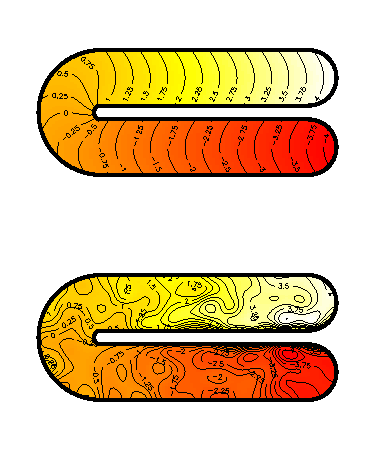
\includegraphics{figs/ramsay-leak.pdf}\\
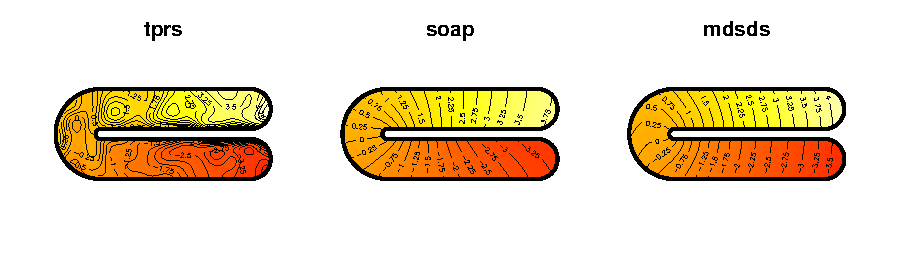
\includegraphics[width=0.45\textwidth]{examples/ramsay/ramsay-real.pdf}\\
%\caption{An example of leakage on the (modified) Ramsay horseshoe (referred to simply as the Ramsay horseshoe here; Wood et al, 2008). A thin plate regression spline was fit to data sampled from the function on the top, the model smooths across the gap in the middle of the domain (bottom).}
\caption{From top to bottom: the modified Ramsay horseshoe function. Below: predictions from models using thin plate regression splines (``tprs''), MDSDS (``mdsds''), the soap film smoother (``soap'') and geodesic low-rank thin plate splines (``gltps'') when 600 points were sampled from the horseshoe and standard normal noise was added. Note that the predictions from the thin plate regression spline fit shows severe leakage.}
\label{leakage}
\end{figure}


The problem of leakage arises because spatial smoothers are based on the idea that data from nearby locations should be similar, but in almost all cases the smoothers measure distance between locations using straight line (Euclidean) distance. This approach is flawed in cases in which straight-line distance is not a meaningful measure of proximity. For example, since whales are not good at travelling on land, the meaningful distance between two whales on either side of the Antarctic peninsula is not the straight line distance across the peninsula, but the shortest path between them that stays entirely in open water. This issue is ubiquitous in spatial ecology. Natural and man-made barriers carve up the landscape (and seascape), partitioning biological populations and spatial models should take this into account. 

In this paper we propose a general method for smoothing, based on generalized distances between points. We apply this to produce a finite area smoother, based on the \textit{within-area distances} between points in the domain of interest. The general approach uses multi-dimensional scaling (MDS; e.g. Chatfield and Collins, 1980, Chapter 10) to associate a location in a $\cal D$ dimensional Euclidian space ({\em p-space}) with each original data point. This is done so that the Euclidian distances between points in p-space approximates the original generalized distance between the points. Smoothing is then performed with respect to locations in p-space. However, reasonable approximation of the generalized distances by the Euclidian distances in p-space can require $\cal D$ to be greater than the 2-4 dimensions in which conventional multi-dimensional smoothers work well. For this reason we revisit the general class of smoothers proposed in Duchon's (1977) thin plate spline paper, selecting a smoother that behaves well with increasing dimension. Note that when applied to the finite area problem our our generalized distance smoother can be viewed as an extension of Wang and Ranalli (2007), which we argue below is somewhat better founded.

The smoother proposed here has the attractive property of being representable using a linear basis expansion with an associate quadratic penalty. Such basis-penalty smoothers have a dual interpretation as Gaussian random fields (eg Rue and Held, 2005), and are appealing because of the ease with which they can be incorporated as components of other models  
(see e.g. Ruppert, Wand and Carroll, 2003 or Wood, 2006 for overviews). Before presenting our proposed method in detail we now briefly review spline type spatial smoothers, and previous approaches to the finite area smoothing problem.

\subsection{Spline smoothing for spatial data}

In the simplest case, we wish to find an $f$ which is a smooth function of spatial coordinates, $x_1$ and $x_2$. We model $f$ using a basis function expansion:
\begin{equation}
f(x_{1}, x_{2}) = \sum_{k=1}^K \beta_k b_k(x_{1}, x_{2}),
\label{basis-exp}
\end{equation}
where the $\beta_k$s are coefficients to be estimated and the $b_k$s are flexible (known) basis functions, such as thin plate spline basis functions or tensor products of B-splines. 

If $K$ is made large enough to avoid substantial model mis-specification bias, then the estimates of $f$ are almost certain to over-fit any data to which they are fitted. For this reason it is usual to associate a measure $J(f)$ of function wigginess with $f$, and to use this to penalize over fit during model estimation. 
For example, consider the simple generalized linear model  
$$
y_i \sim \text{EF}(\mu_i, \phi),~~~~ g(\mu_i) = \eta_i =f(x_{1i},x_{2i})
$$
where EF denotes an exponential family distribution with mean $\mu_i$ and scale parameter $\phi$, while $g$ is a known link function and $\eta_i$ is known as the `linear predictor' of $y_i$. Letting $l({\bm \beta})$ be the log likelihood then estimation of $\bm \beta$ is by maximization of 
$$
l({\bm \beta}) - \lambda/2 J(f)
$$ 
where $\lambda$ is a tune-able smoothing parameter, used to control the wiggliness of the estimate of $f$ $\lambda $ is typically estimated by GCV or marginal likelihood maximization (see e.g. Wood, 2011). A popular $J(f)$ in the spatial context is the 2 dimensional thin plate spline penalty
$$
J(f) = \int \left (\pdif{^2 f}{x_1^2}\right )^2 + 2\left ( \pddif{f}{x_1}{x_2}\right )^2 + \left (\pdif{^2 f}{x_2^2}\right )^2 dx_1 dx_2
$$
which can conveniently be written as a quadratic form in $\bm \beta$. 

Within this framework it is straightforward to allow $\eta_i$ to depend on multiple smooth functions of various predictor variables, as well as on conventional parametric terms that are linear in any unknown parameters (e.g. Wood, 2006, based on Hastie and Tibshirani, 1990). Such models are widely used in quantitative ecology, for example in the creation density maps which can then be integrated over the domain to obtain an abundance estimate (see e.g.  Hedley and Buckland, 2004; Williams et al, 2011) or as part of a larger model, taking into account nuisance spatial effects (e.g. Augustin et al, 2009). 

\section{Previous approaches to the problem of leakage}
\label{previous-approaches}

There 3 main types of existing approach to dealing with the finite area smoothing problem.

\subsection*{Partial differential equation methods}

Ramsay (2002) exploited the link between smoothing with differential operator based penalties and Partial Differential Equations to produce a smoother defined as the solution to a particular PDE problem defined only over a finite area. His FELSPINE method uses a finite element method to compute a smoother, based on the penalty 
\beq
J(f) = \int_\Omega \left ( \pdif{^2 f}{x_1^2} + \pdif{^2 f}{x_2^2} \right )^2 dx_1 dx_2 
\label{soap}
\eeq 
Where $\Omega$ is the region of the $x_1$, $x_2$ plane of interest. Ramsay had to use the very strong boundary condition that contours of $f$ meet the boundary of $\Omega$ at right angles, which leads to artefacts when the condition does no hold (see Wood, Bravington and Hedley, 2008). The computational method also makes it awkward to include such terms in larger models.

Wood et al (2008) use the physical analogy of a soap film to motivate an alternative which can be represented as a basis penalty smoother, and has better boundary behaviour. First consider the domain boundary to be made of wire, then dip this wire into a bucket of soapy water; a soap film with the same shape as the boundary will have then formed. If the wire lies in the spatial plane, the height of the soap film at a given point is the values of the smooth at that point. This film is then distorted smoothly toward each datum, while minimising the overall surface tension in the film. Mathematically the soap film consists of two sets of basis functions, one that is based entirely inside the domain (a set of interior knot locations are specified) and one that is induced by the (known or estimated) boundary values. These functions are found by solving Poisson and Laplace's equations in two dimensions. The penalty associated with the former set is again (\ref{soap}). 

The soap film approach has the basis-penalty form that is convenient for applied work and solves the boundary leakage problem, but basis setup is quite computationally expensive, and for many applications the approach is less natural than smoothing using within domain distances. A further problem with the soap film approach is that no distinction exists between `open' boundaries (for example a boundary that is simply the edge of a survey region) and `hard' boundaries (real physical barriers).  

\subsection*{Within area distances}

Wang and Ranalli (2007) propose to replace straight-line distances with `geodesic' distances in a smoother that is a sort of approximate thin plate spline. To calculate the geodesic distances, a graph is constructed in which each vertex is the location of an observation and is only connected to its $k$ nearest neighbours. The within area distances between each vertex pair is approximated using  Floyd's algorithm (Floyd, 1962) to find the shortest path through the graph. This algorithm is cubic in the number of data, making the approach very costly for large datasets. At large sample sizes the geodesic distances will tend towards `within area distance', i.e. the shortest path between two point that lies entirely within the domain of interest (see Bernstein et al, 2000). 

Wang and Ranalli use their geodesic distances in place of the usual Euclidian distances in the radial basis functions used to define a thin plate spline. They leave the basis for the null space of the thin plate spline penalty unchanged, so that some linkage across boundary features remains in the smoother. The principle difficulty in interpreting the results of their method is that it is unclear what their penalty term penalizes. The interpretational difficulty arises because  Wang and Ranalli's expressions (3) and (9) involve the square roots of matrices that are not positive semi-definite. In the case of their expression (3), which relates to a thin plate spline, this problem would be rectifiable if the spline coefficients had the usual thin plate spline linear constraints applied in order to force positive definiteness on the spline penalty. However in the case of (9), which defines their geodesic splines, there appears to be no sensible way to obtain positive semi-definiteness. This is a problem because matrix square roots in general only exist for positive semi-definite matrices plus some rather special cases not useful here (see e.g. Higham, 1987). It appears that for computational purposes Wang and Ranalli have used the generalization of a matrix square root given in appendix A.2.11 of Ruppert, Wand and Carroll (2003), but this square root lacks the basic properties that would allow Wang and Ranalli's (2) to be interpretable exactly as a thin plate spline, or for it to be possible to work out what the penalty on their geodesic spline is actually penalizing. 

The method appears to work well in simulations. However, the combination of an un-modified null space, the opacity of the penalty meaning and $O(n^3)$ computational cost are of some concern for practical work. For these reasons it seems worthwhile to try and come up with alternative ways of using the within area distance idea, while avoiding these difficulties. 

\subsection*{Domain warping}


Paul Eilers (in a seminar at University of Munich in 2006) suggested conformally mapping the smoothing domain to a convex one  via the Schwarz-Christoffel transformation (Driscoll and Trefethen, 2002). The idea is that smoothing can then be conducted on the convex domain, without leakage problems. The first author has extensively investigated such an approach (Miller, 2011, Chapter 3), but there are insurmountable difficulties associated with the extreme modification of inter-observation distances necessary to achieve domain convexity, which cause artefacts that are significantly more problematic than the leakage effects that the method seeks to avoid. 

The methods proposed in the next section can be viewed as an attempt to put within area distance methods on a more interpretable foundation by using an extension of the notion of domain warping. 


\section{The generalized distance smoothing model}
\label{proposed-model}

We assume that we want to model a response $y_i$ which is dependent on covariates via a linear predictor $\eta_i$. Our model is then
$$
\eta_i = \alpha_i + f({\bf d}_i)
$$
where $\alpha_i$ may depend linearly on further model coefficients (or may simply be zero). $f$ is a smooth function, dependent on ${\bf d}_i$, a vector of generalized distances between the $i^{\rm th}$ observation and either i) the other observations, or ii) some set of `reference points'. 

We complete the model by setting 
$$
f({\bf d}_i) = f_{\cal D}\{{\bf x}({\bf d}_i)\}
$$
where ${\bf x}({\bf d})$ is the location of the point with distance vector $\bf d$ in the $\cal D$ dimensional 
Euclidean space determined by multi dimensional scaling applied to either i) the matrix for the complete data set or ii) the distance matrix for the set `reference points' referred to above. $f_{\cal D}$ is a $\cal D$ dimensional `Duchon-spline' (Duchon 1977), a generalization of the familiar thin plate spline. 

The key idea here is that we smooth over a Euclidean space  in which the Euclidean inter-observation distances are approximately equal to the original generalized distances. That is  $\|{\bf x}({\bf d}_i) - {\bf x}({\bf d}_j) \| \approx d_{ij}$ when $d_{ij}$ is the generalized distance between points $i$ and $j$ ($\|\cdot \|$ is the Euclidean norm). The choice of $\cal D$ determines the accuracy of the distance approximation. This can either be part of model specification, in which case $\cal D$ is chosen to achieve some specified level of approximation accuracy, or more pragmatically, can be chosen to optimize estimated prediction error (e.g. to optimize GCV).

In the case of finite area smoothing, the elements of ${\bf d}_i$ are `within area' distances between points, that is to say the shortest path between two points, such that the path lies entirely within the domain of interest. We will refer to the original 2 dimensional data co-ordinates as being elements of the `o-space' while $\cal D$ dimensional co-ordinates in the MDS projection will be referred to as elements of the `p-space'. Appendix B gives and algorithm for calculating within-area distances for simple polygons. 

These smoothers will be henceforth referred to as MDSDS (Multi Dimensional Scaled Duchon Splines), and the next three subsections provide the details for the MDS, smoothing and $\cal D$ selection steps.

\subsection{MDS as a transformation of space}

In this section we consider the construction of the mapping ${\bf x}({\bf d})$ by multi-dimensional scaling (MDS; Gower, 1966). We start the process by choosing a representative set of locations of size $n_s$ within the domain of interest (i.e. in o-space). This set might be all the locations at which we have observations, but in the case of finite area smoothing we would usually choose a set of locations spread uniformly over the region of interest, in order to ensure that all the important geographic features in o-space will be represented in p-space. 

The generalized distances between all pairs of points in the representative set are then computed, in order to obtain a matrix $\bf D$ such that $D_{ij}$ is the squared generalized distance between points $i$ and $j$. MDS then finds a configuration of points in $\cal D$ dimensions Euclidean space such that the Euclidean distances between the points approximate the original generalized distances. The recipe for achieving this is straightforward. Defining ${\bf H} = {\bf I} - {\bf 11}\ts/n_s$ we can obtain the double centred version of $D$, ${\bf S} = - {\bf HDH}/2$, which is then eigen-decomposed
$$
{\bf S} = {\bf U}{\bm \Lambda}{\bf U}\ts.
$$ 
The rows of  ${\bf X }= {\bf U}{\bm \Lambda}^{1/2}$ then give locations in an $n_s$ dimensional Euclidean space, such that the interpoint Euclidean distances in that space match the original generalized distances. In practice, dimension reduction is required, so we retain only the first $\cal D$ columns of $\bf X$ to create our p-space, accepting that the interpoint distances in this $\cal D$ dimensional space will only approximate the original generalized distances. See e.g. Chatfield and Collins (1980, Chapter 10) for more details.

We then require some means for finding the location in p-space of a point in o-space that was not in the original representative set used in $\bf D$. Let $\bf d$ be the $n_s$ vector of squared generalized distances (in o-space) between this new point and the points in the original representative set. Gower (1968) gives the following interpolation formula for the location of the new point in p-space 
$$
{\bf x} = - {\bm \Lambda}^{-1/2} {\bf U}\ts {\bf d}^\prime
$$
where $d^\prime_i = d_i - S_{ii}$. Again, $\bf x$ would usually be truncated, retaining only its first $\cal D $ components. 

So, MDS combined with Gower's interpolation formula provide a means for constructing and computing with ${\bf x}({\bf d})$. We now turn to the construction of a suitable smoother in p-space.



\subsection{Smoothing with Duchon splines}
\label{ss:duchon}

In order for our smoother to have a convenient basis-penalty form, we need to smooth in p-space using a basis-penalty smoother. A thin plate spline (TPS) is the obvious choice for smoothing arbitrarily scattered data where the Euclidean distance between points determines similarity, but there is a technical problem. To achieve a smooth $f$ requires $2m > {\cal D}$ where $m$ is the order of differentiation in the TPS penalty, but the dimension of the space of unpenalized functions in a TPS basis is 
$ M = \left ( \begin{array}{c} m + {\cal D} - 1 \\ {\cal D} \end{array} \right )$. As figure \ref{nullspace-dim} shows the minimum possible $M$ increases rapidly with $\cal D$, leading to the danger of substantial undersmoothing as $\cal D$ increases.

\begin{figure}
\centering
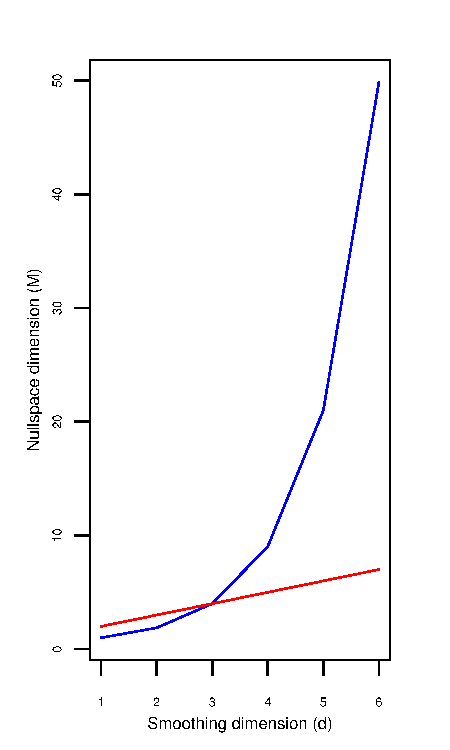
\includegraphics[width=3in]{figs/nullspace-dim.pdf} \\
\caption{Relationship between smoothing dimension ($d$) and the nullspace dimension ($M$) when $m$ (the derivative penalty order) is set to 2 for thin plate regression splines (dashed) and Duchon splines (solid). Note that as the nullspace dimension increases, the complexity of those functions in the nullspace increases too. For the thin plate splines a combination of the continuity condition that $2m>d$ and the form of $M$ (see (\ref{gds-bigm})) makes the size of the nullspace increase very quickly with smoothing dimension.}
\label{nullspace-dim}
% generated by thesis/mds/figs/nullspace-dim.R
\end{figure}


To combat this problem we propose to use a smoother from the larger class of functions considered in Duchon's (1977) paper introducing thin plate splines, which will allow us to obtain a smoother for which $M = {\cal D} + 1$. This larger class has been almost entirely ignored in the statistical literature, so we provide a brief summary here. 

The difference between general Duchon splines and thin plate splines is in the smoothing penalty used. To understand the difference it helps to start with the general TPS penalty
\begin{equation}
J_{m,{\cal D}} = \int_{\mathbb{R}^d} \sum_{\nu_1 + \dots + \nu_d=m} \frac{m!}{\nu_1! \dots \nu_d!} \left( \frac{\partial^m f \left (\mathbf{x} \right )}{\partial x_1^{\nu_1} \ldots  \partial x_d^{\nu_d}} \right)^2 \text{d} x_1 \ldots  \text{d} x_d.
\label{tprs-pen}
\end{equation}
By Plancherel's theorem (e.g. Vretblad, 2003, p. 180), if we take the Fourier transform, $\mathfrak{F}$, of the derivatives in (\ref{tprs-pen}) then the penalty can be re-expressed as
\begin{equation}
J_{m,{\cal D}} =  \int_{\mathbb{R}^d} \sum_{\nu_1 + \dots + \nu_d=m} \frac{m!}{\nu_1! \dots \nu_d!} \left ( \mathfrak{F} \frac{\partial^m f}{\partial x_1^{\nu_1} \ldots  \partial x_d^{\nu_d}} \left (  \boldsymbol{\tau}\right ) \right )^2 \text{d} \boldsymbol{\tau}.
\label{tprs-pen-ft}
\end{equation}
where $\bm \tau$ are now frequencies, rather than locations. Duchon then considers weighting the Fourier transform of the derivatives by some power of frequency, effectively increasing the penalization of high frequency components in the spatial derivatives if the power is positive. The resulting penalty is 
\begin{equation}
\breve{J}_{m,{\cal D}} = \int_{\mathbb{R}^d} \| \boldsymbol{\tau} \|^{2s} \sum_{\nu_1 + \dots + \nu_d=m} \frac{m!}{\nu_1! \dots \nu_d!}\left ( \mathfrak{F} \frac{\partial^m f}{\partial x_1^{\nu_1} \ldots  \partial x_d^{\nu_d}} \left (\boldsymbol{\tau} \right ) \right )^2 \text{d} \boldsymbol{\tau}.
\label{duchon-penalty}
\end{equation}
where $-{\cal D} < 2s < {\cal D}$ and the restriction $m + s > {\cal D}/2$ is applied to ensure continuity of the splines that result from use of this penalty. 

Duchon shows that the function minimising (\ref{duchon-penalty}) while interpolating or smoothing data at locations ${\bf x}_i$ has the form 
$$
\hat f({\bf x}) = \sum_i^n \gamma_i K_{2m+2s-{\cal D}}(\|{\bf x}-{\bf x}_i\|) + \sum_j^M \alpha_j \phi_j({\bf x})
$$
where the $\phi_j({\bf x})$ form a basis for the polynomials of order $<m$, ${\bf x}_i$ is the ith observation location and $\gamma_i$ and $\alpha_j$ are coefficients to be estimated, subject to the $M$ linear constraints
\beq
\sum_i^n \gamma_i \phi_j({\bf x}_i)=0.
\label{duchon.constraint}
\eeq
The other basis functions are given by
$$
K_d(t) = \left \{ \begin{array}{ll}
(-1)^{(d+1)/2}|t|^d & d \text{~~odd}\\
(-1)^{d/2}|t|^d\log |t| & d \text{~~even}
\end{array} \right .
$$
Finally, given the linear constraints (\ref{duchon.constraint}),
$$
\breve{J}_{m,{\cal D}} = {\bf \delta} \ts {\bf K} {\bf \delta}
$$
where $K_{ij} = K_{2m+2s-{\cal D}}(\|{\bf x}_i-{\bf x}_j\|)$. Notice that $s=0$ gives a conventional TPS.

As an example of using this basis and penalty, we note that estimating $f$ to minimize
$$
\sum_i^n (y_i - f({\bf x}_i))^2 + \lambda \breve{J}_{m,{\cal D}}
$$
now reduces to the straightforward optimization problem of finding $\hat {\bm \gamma} $ and $\hat {\bm \alpha}$ to minimize
$$
\|{\bf y} - {\bf K } {\bm \gamma} - {\bf A}{\bm \alpha}  \|^2 + \lambda {\bm \gamma}\ts {\bf K} {\bm \gamma} ~~\text{s.t.}~~{\bf A}\ts {\bm \gamma} = {\bf 0}
$$
where $A_{ij} = \phi_j({\bf x}_i)$. Notice that this problem has exactly the same structure as the TPS problem, so exactly the same approach to computation can be taken. More importantly optimal rank reduced versions of these Duchon splines can be produced using the methods given in Wood (2003) for the TPS. Wood (2003) uses an eigen approximation to the full spline thereby avoiding the difficult problem of $\cal D$ dimensional knot placement that complicates other approaches to reduced rank splines, so we use this approach in what follows.

We are now in a position to produce a spline suitable for smoothing in p-space. Specifically we choose a (reduced rank) Duchon spline with $m=2$ and $s = {\cal D}/2 - 1$, which will give us a smooth $f$ for which $M={\cal D}+1$ (i.e. the unpenalized component of $f$ grows only linearly with $\cal D$).

 


\subsection{Selecting $\cal D$}
\label{s:mdsdimselect}

An obvious question is whether we actually need $\cal D$ to be larger than 2 in practice. Figure \ref{wt2-plot} provides an illustration that in general we do. It shows what happens when within area distances over a 2 dimensional domain with a peninsulae are used to obtain a 2D p-space. Some of the points in the resulting p-space configuration become quite severely squashed together. In fact truncating the projection to two dimensions can sometimes cause the basic ordering of the points to be lost, making the task of the smoother impossible. Further investigation showed that increasing the dimensionality of $p$-space maintains the ordering of the points, however the number of dimensions required varied according to the shape of the domain. 

\begin{figure}
\centering
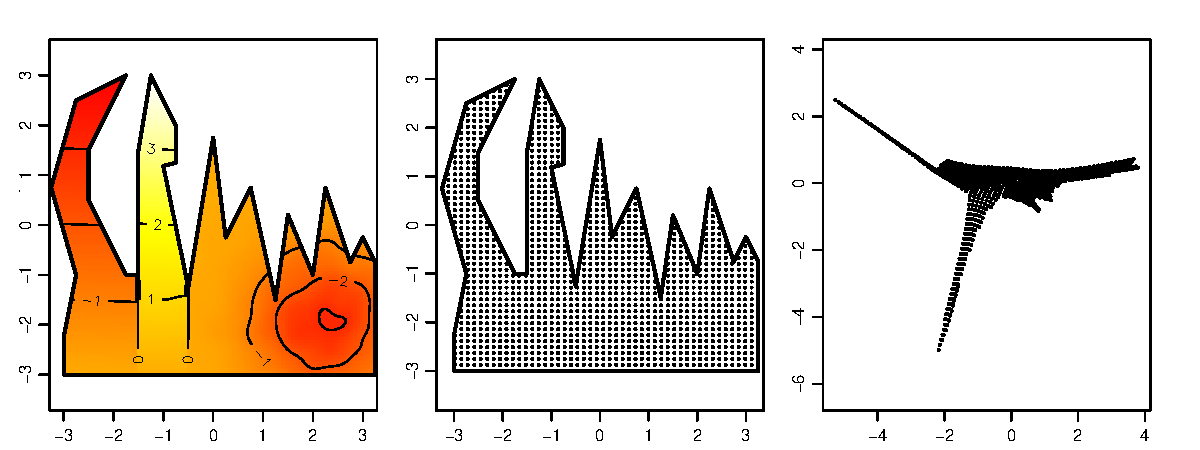
\includegraphics[width=\textwidth]{examples/wt2/wt2-plot.pdf} \\
\caption{Left to right: surface of the peninsulae domain, points in the domain and finally their projection into 2-dimensional MDS space when within-area distances are used to calculate the distance matrix. The MDS space plot shows that some squashing can happen in two dimensions. The large left peninsula and some of the smaller peninsulae have lost their ``width'' and, in fact, points within them have lost ordering.}
\label{wt2-plot}
% generated by examples/wt2/wt2-plot.R
\end{figure}

Having accepted the need for ${\cal D}>2$, we need some means for choosing $\cal D$. The two obvious strategies might be characterised as `model driven' and `data driven'. 

In the model driven approach we specify the accuracy with which the inter-point distances in p-space must match the original generalized distances as part of model specification, and $\cal D$ is then increased during fitting until this specification is met. In the data driven approach then $\cal D$ is chosen in order to optimize some prediction error criterion, such as GCV.  Figure \ref{aral-gcvplot} shows the relationship between $\cal D$ and GCV score for the Aral sea data analysed below.

Notice that selecting $\cal D$ is typically a small part of the computational burden, since the MDS and smoothing are usually cheap relative to the computation of distances (at least in the finite area smoothing case).


\section{Examples}
\label{examples}

To illustrate the utility of the model two simulation studies are shown, followed by examples using real data. All concentrate on the finite area smoothing problem. In each case MDSDS was compared with thin plate splines (which do not account for the boundary), geodedic low-rank thin plate splines (GLTPS) and the soap film smoother (which both do account for the boundary). The GLTPS model was as described in Wang and Ranalli (2007), but with the within-area distances calculated as described in Appendix B (i.e. the same as for MDSDS); knots were placed using the \texttt{cover.design} method in the package \texttt{fields} (again, as in Wang and Ranalli (2007)). In all cases smoothing parameters were selected by GCV. The \textsf{R} packages \texttt{mgcv} (available from CRAN), \texttt{soap} (available from \url{http://www.maths.bath.ac.uk/~sw283/simon/software.html}) and \texttt{msg} (available from \url{https://github.com/dill/msg}) were used to fit the models. Code for fitting the GLTPS is available at \url{https://github.com/dill/gltps}

In all the cases below the basis size specified refers to the maximum basis size allowed, since the penalty will reduce the complexity of the smoother, we simply need to specify an upper bound on the basis size.


\subsection{Ramsay's horseshoe}

The horseshoe shape shown in the top panel of Figure \ref{leakage} is an obvious benchmark for techniques that wish to combat leakage. Although perhaps unrealistic (and bordering on pathological), any new method that works well on the horseshoe should have a good chance of working well in more realistic situations. A simulation experiment was run with the same setup as in Wood et al. (2008): 200 replicates were generated at each of three error levels (standard normal noise multiplied by 0.1, 1 and 10) with sample size 600. A thin plate regression spline, (Wood, 2003), with basis size 100 and a soap film smoother with 32 interior knots  and a 40 knot cyclic  spline was used to estimate the boundary. For the MDSDS model, the basis size was set to 100 and a 20 by 20 initial grid was used for the MDS projection (see Appendix A), MDS projection dimension was selected by GCV in the range of 2 and the number of dimensions that explained 95\% of the variation in the distance matrix of the initial grid. For the GLTPS 40 knot locations were selected as in Wang and Ranalli (2007). For each realisation the mean squared error (MSE) was calculated between the true function and a prediction grid of 720 points.

\begin{figure}
\centering
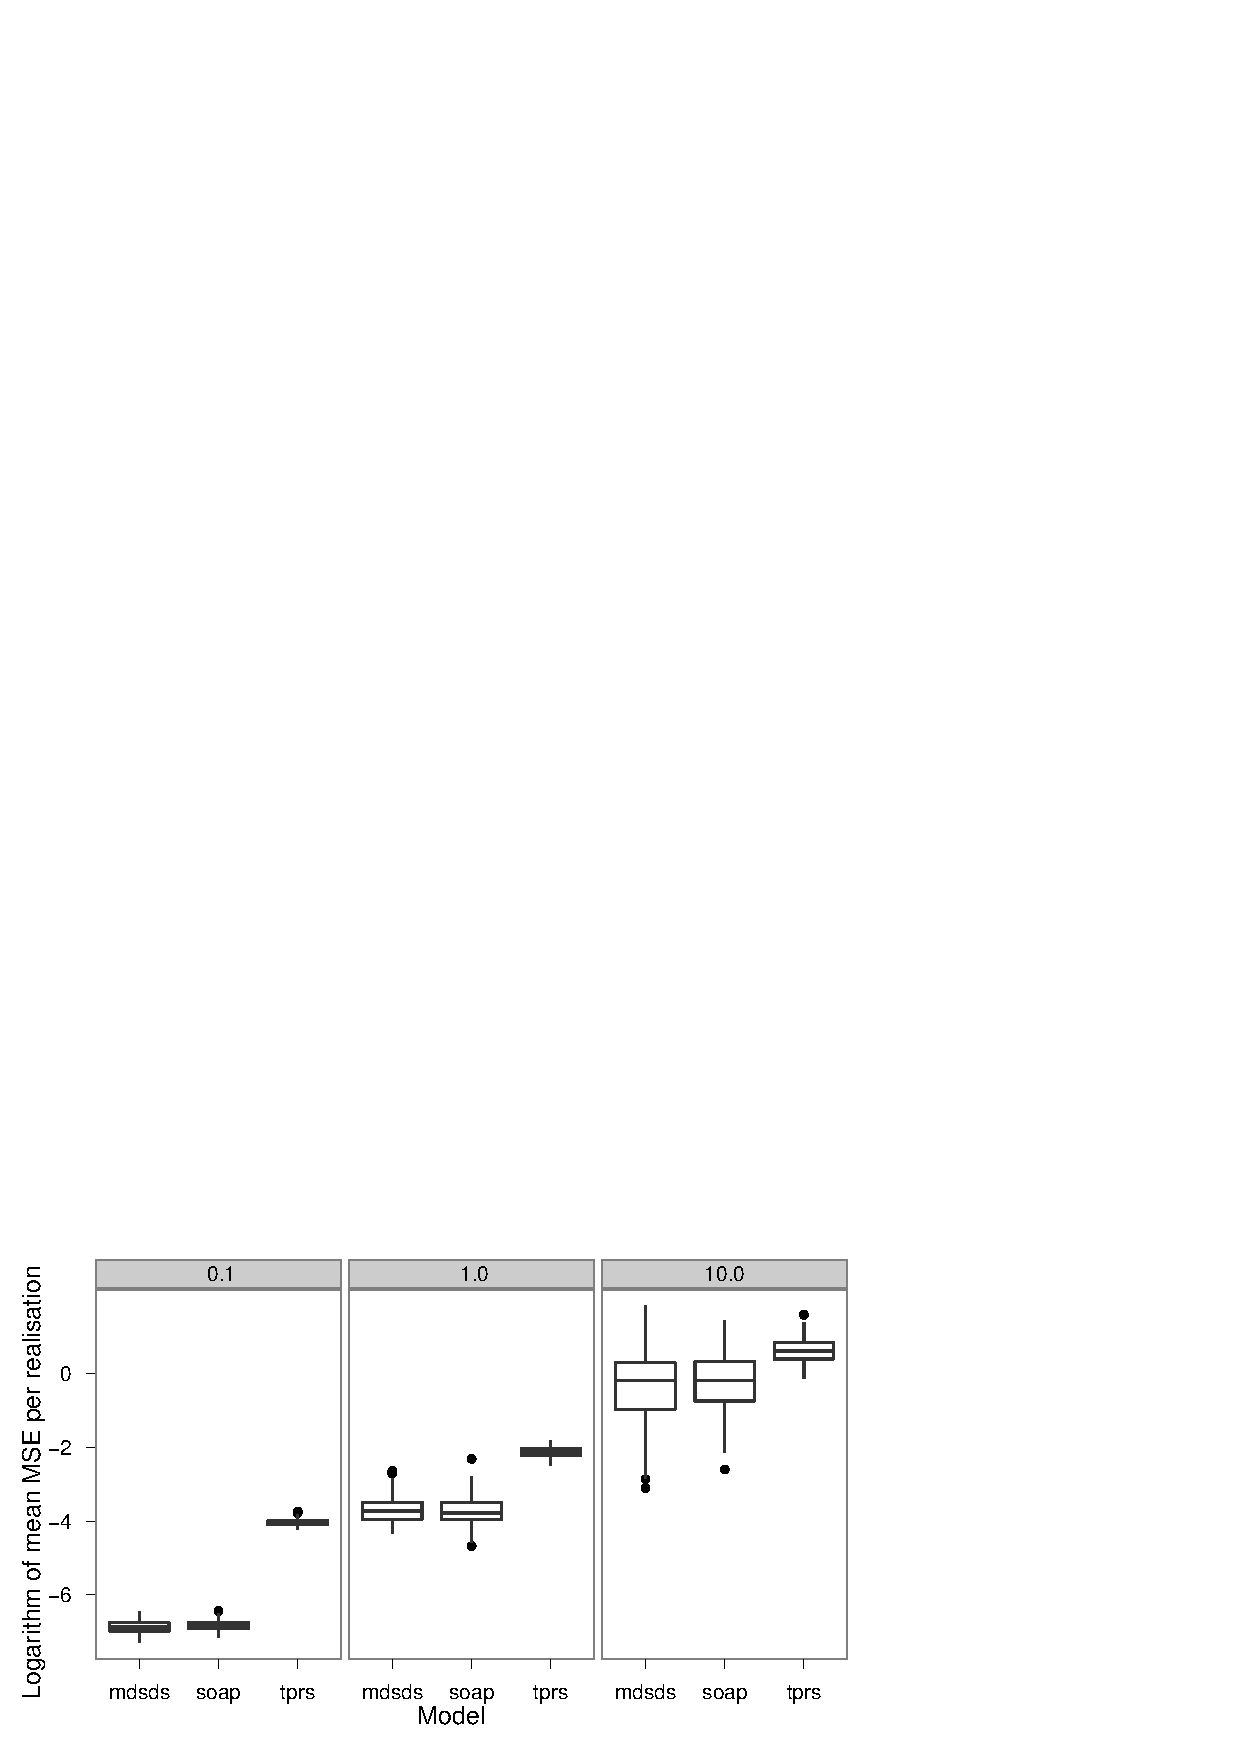
\includegraphics[width=\textwidth]{examples/ramsay/ramsay-result.pdf}
%\caption{Top: boxplots of per-realisation $\log$ mean squared error at the three noise levels. Using a paired Wilcoxon signed two-sample test, the difference between the new approach (``mdsds'') and the other models was significantly different for the two lower noise levels (at the 0.05 level). For the higher noise level, the three methods that accounted for the boundary (``gltps'' and ``soap'') were not distinguishable from MDSDS. The thin plate regression spline (``tprs'') was worse.
\label{ramsay-results}
% generated by examples/ramsay/ramsay-plot.R
\end{figure}

As can be seen in Figure \ref{ramsay-results}, the thin plate regression spline has rather poor performance in MSE terms while MDSDS, the soap film smoother and GLTPS perform significantly better. MDSDS outperforms the soap film and GLTPS at lower noise levels, becoming indistinguishable at the highest noise level. The median number of dimensions selected for the MDS projection using GCV was 3 (max. 14, min. 2). Looking more qualitatively at the bottom three plots in Figure \ref{ramsay-results}, the predictions do not show any evidence of leakage.

% Wilcoxon vs. MDSDS
%tprs noise= 0.1 -1 p= 1.447002e-34 
%soap noise= 0.1 -1 p= 7.672467e-07 
%gltps noise= 0.1 -1 p= 1.447002e-34 
%tprs noise= 1 -1 p= 1.447002e-34 
%soap noise= 1 1 p= 0.003321106 
%gltps noise= 1 1 p= 0.0003642348 
%tprs noise= 10 -1 p= 5.060672e-25 
%soap noise= 10 -1 p= 0.8533422 
%gltps noise= 10 -1 p= 0.05883376 

\subsection{Peninsulae}

The results from the modified Ramsay horseshoe are encouraging. However, as mentioned above, the domain is not particularly realistic. To further explore the performance of MDSDS a more realistic domain was used. The domain, which attempts to mimic a coastline, is shown in the left panel of Figure \ref{wt2-plot}.

Simulations were run at a series of noise levels 0.35, 0.9 and 1.55 equating to signal-to-noise ratios of 0.50, 0.75 and 0.95, respectively. The soap film smoother used 109 internal knots and 60 for the cyclic boundary smooth. The MDSDS models used an initial grid of 120 by 126 points, the basis size was 140. The thin plate regression spline basis size was also 140. For the GLTPS, 80 knots were selected using the space filling design, as above.

Figure \ref{wt2-boxplots} shows the boxplots of the $\log$ of the MSE per realisation for each model. In the low noise cases, a paired Wilcoxon signed rank test showed that the soap film smoother and MDSDS were not significantly different at the 0.05 level. In all cases MDSDS was significantly better than both GLTPS and thin plate regression splines.

% Wilcoxon vs. MDSDS
%tprs noise= 0.35 -1 p= 7.969241e-31 
%gltps noise= 0.35 -1 p= 1.298381e-14 
%soap noise= 0.35 -1 p= 0.1789427 
%tprs noise= 0.9 -1 p= 1.903392e-28 
%gltps noise= 0.9 -1 p= 1.032922e-11 
%soap noise= 0.9 -1 p= 1.23365e-11 
%tprs noise= 1.55 -1 p= 9.46488e-32 
%gltps noise= 1.55 -1 p= 0.01354858 
%soap noise= 1.55 -1 p= 0.01313839 

\begin{figure}
\centering
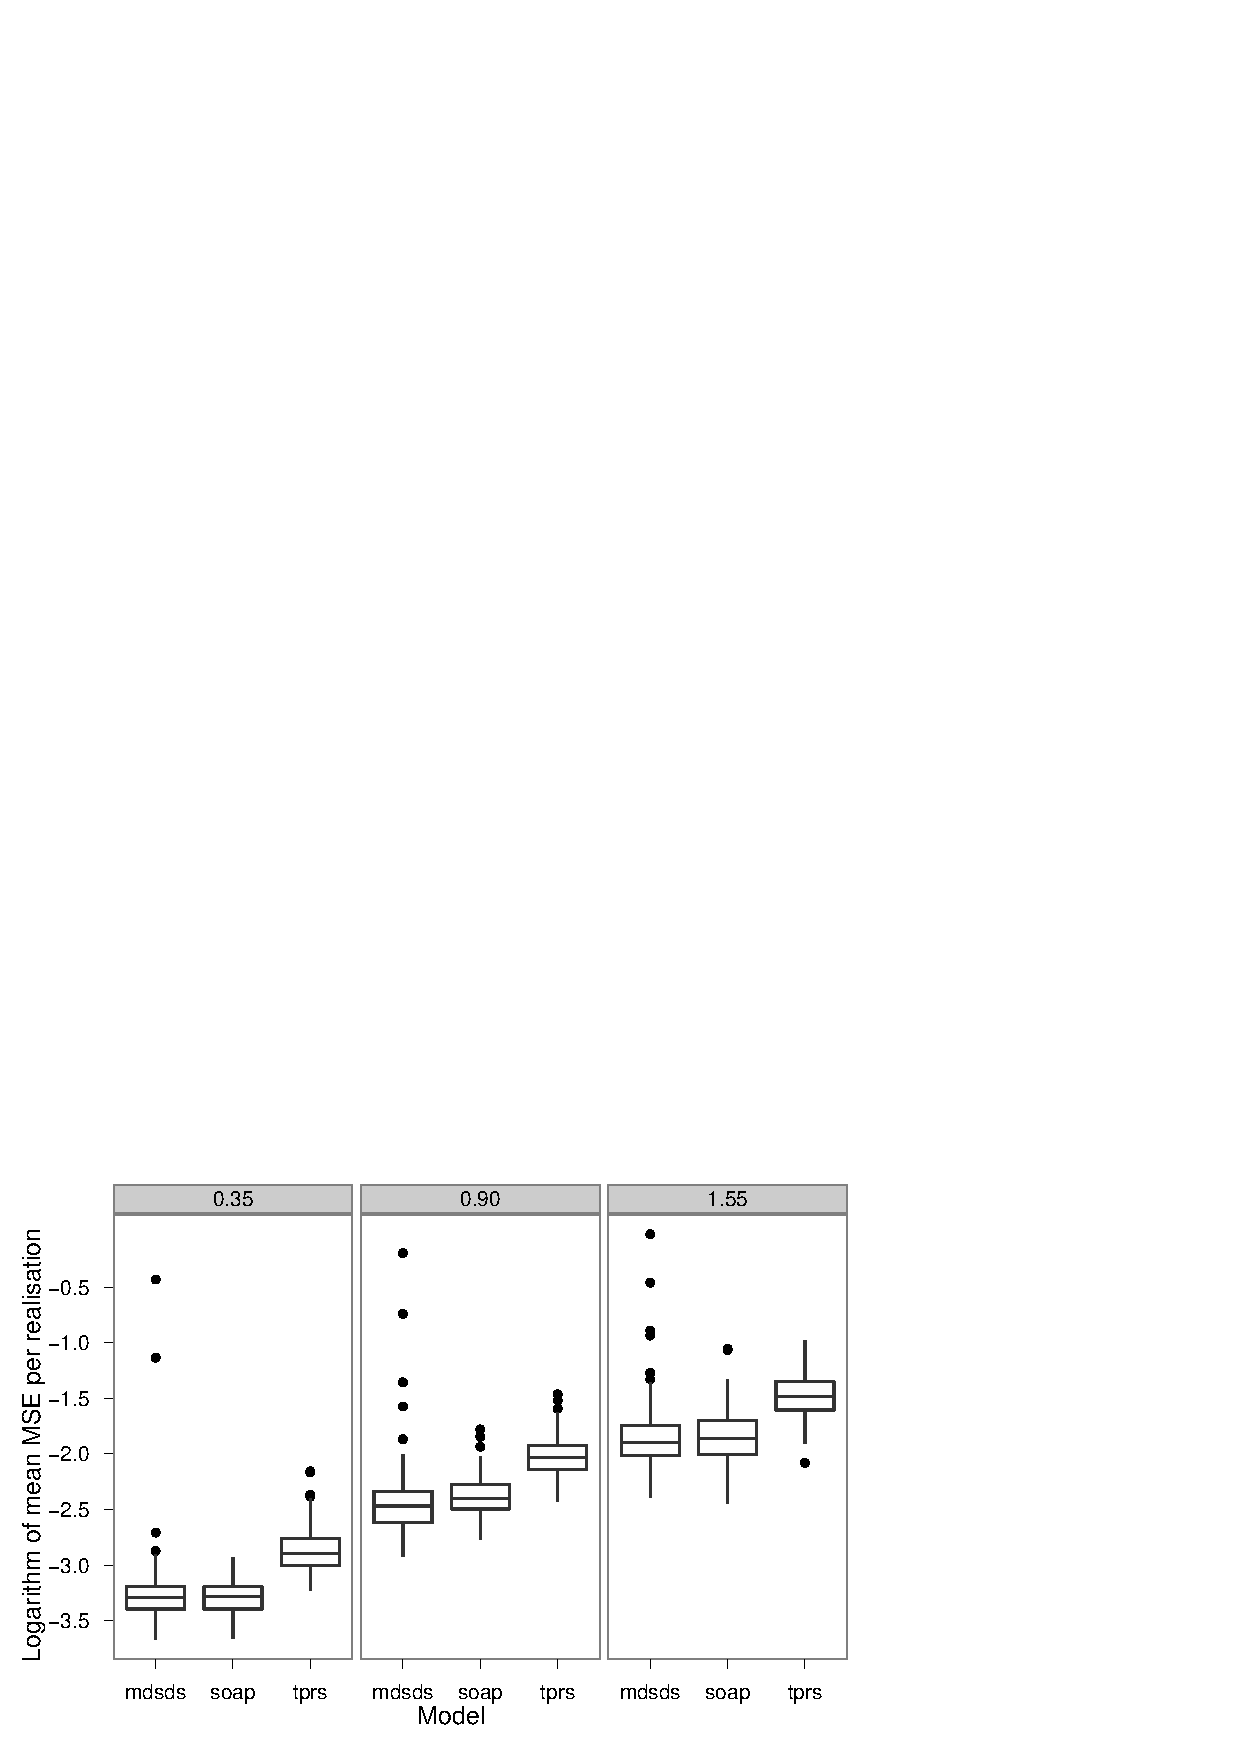
\includegraphics{examples/wt2/wt2-result.pdf} \\
\caption{Boxplots of logarithm of mean MSE per realisation for the models tested on the peninsulae domain at three noise levels. At each noise level, the median mean MSE was lower for MDSDS than for the thin plate regression spline or soap film smoother. A paired Wilcoxon signed rank test showed that the difference between MDSDS and the soap film smoother was only non-significant at the 0.35 noise level.}
\label{wt2-boxplots}
% generated by examples/wt2/wt2-boxplot.R
\end{figure}



\subsection{Aral sea}

The Aral sea is located between Kazakhstan and Uzbekistan. It has been steadily shrinking since the 1960s when the Soviet government diverted the sea's two tributaries in order to irrigate the surrounding desert. The NASA SeaWifs satellite collected data on chlorophyll levels in the Aral sea over a series of 8 day observation periods from 1998 to 2002 (Wood et al, 2008). The 496 data are averages of the $38^\text{th}$ observation period. Smooths were fitted to the spatial coordinates (Northings and Eastings; kilometres from a specified latitude and longitude) with the logarithm of chlorophyll concentration (modelled with a Gamma distribution) as the response.

The models that were fitted to the data were: a thin plate regression spline with basis size 70, MDSDS with a basis size of 70 (a 20 by 20 initial grid was used for the MDS projection) and soap film using 49 boundary knots and 74 internal knots. Using GCV for MDS projection dimension selection lead to a 5-dimensional projection. A plot of the relationship between projection dimension and GCV score can be seen in Figure \ref{aral-gcvplot}; there is a clear minima at 5 dimensions.

\begin{figure}
\centering
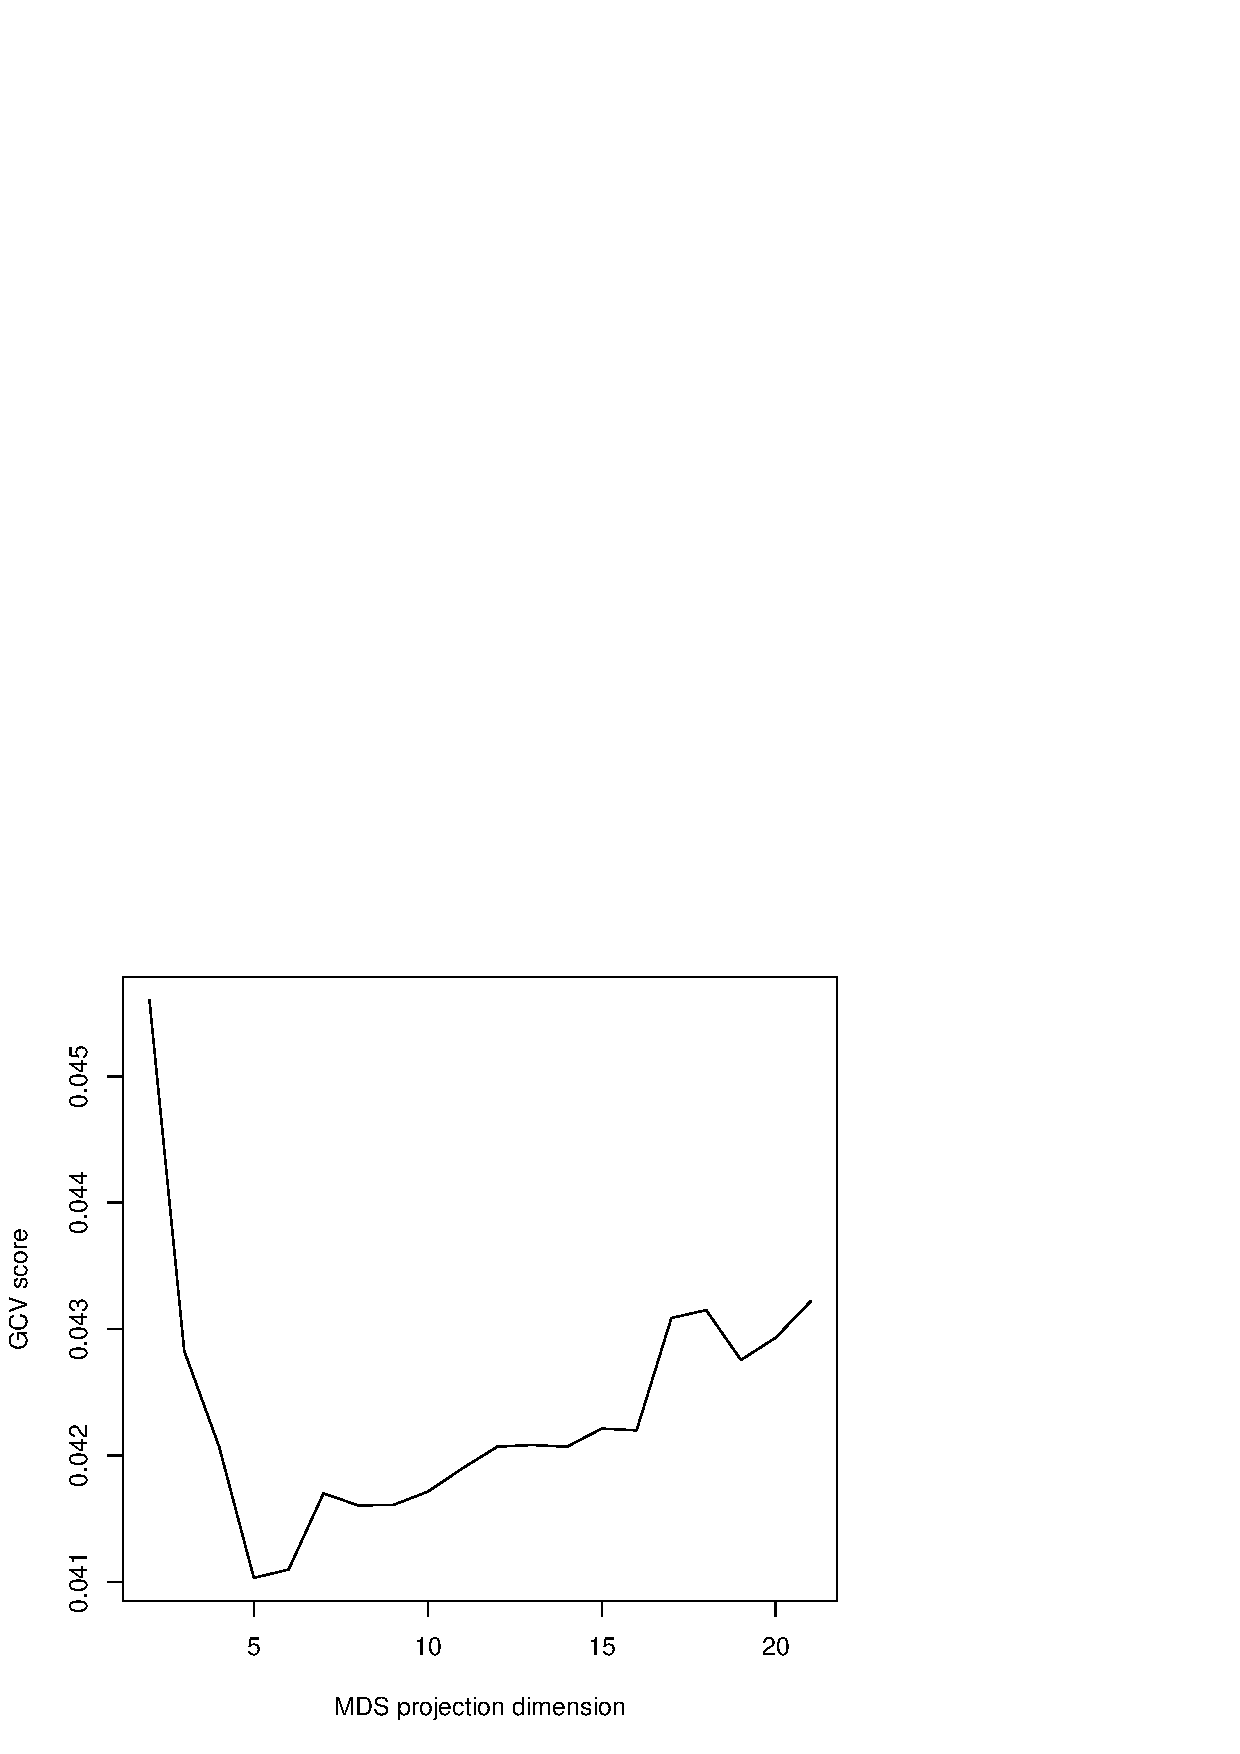
\includegraphics[width=3.5in]{examples/aral/aral-gcvplot.pdf} \\
\caption{Plot of the relationship between GCV score and MDS projection dimension for the Aral sea data set. Here a clear minima at 5 dimensions can be seen, however there is no particular reason to believe that there will always be such a pronounced optima.}
\label{aral-gcvplot}
% generated by examples/aral/aral-plot.R
\end{figure}

Predictions from the models over a grid of 496 points are shown in Figure \ref{aral-plot}. The fits are broadly similar across most of the domain, both MDSDS and the soap film smoother do not show signs of leakage around (-50,-50), as the thin plate regression spline does.



\begin{figure}
\centering
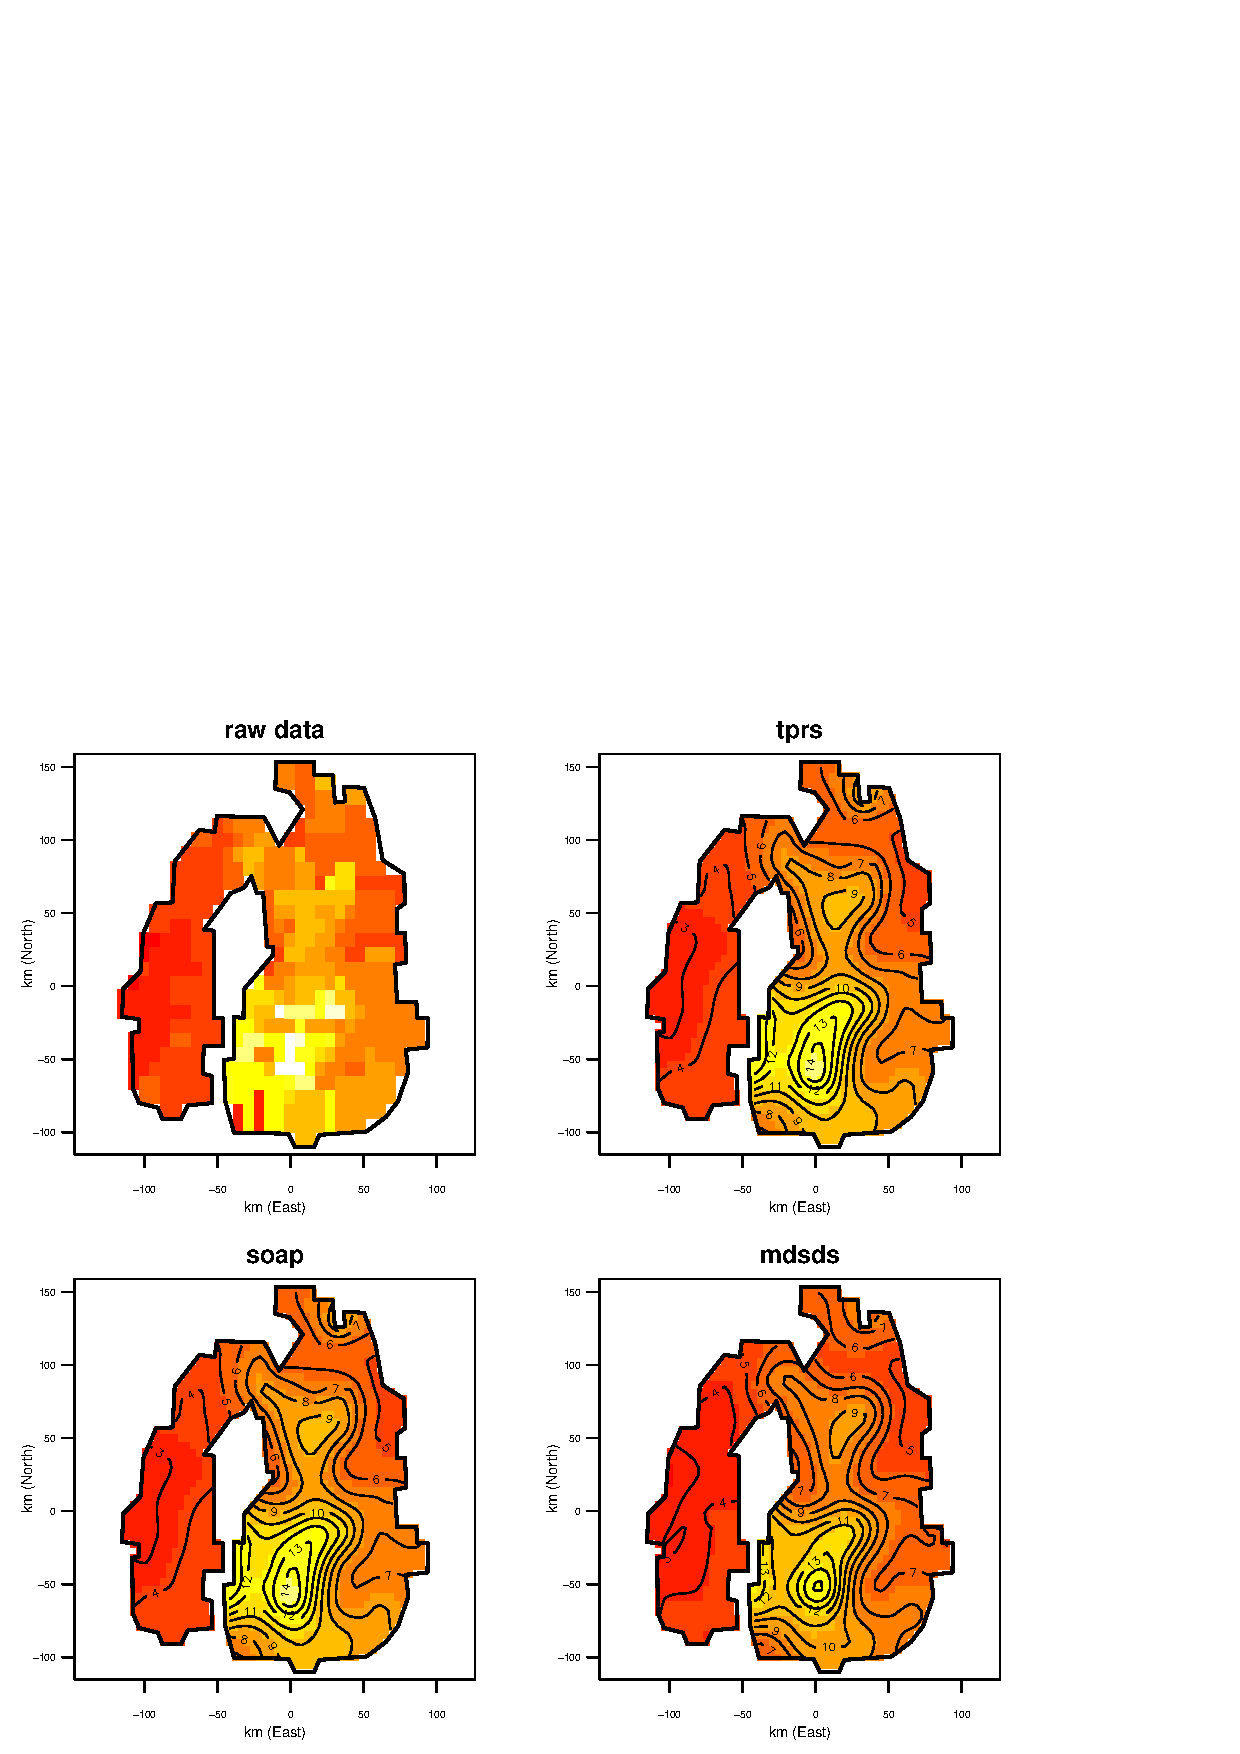
\includegraphics[width=\textwidth]{examples/aral/aral-plot.pdf}
\caption{replace this}
\label{aral-plot}
% generated by examples/aral/aral-plot.R
\end{figure}

%\caption{Aral sea analysis. Clockwise from top left: raw data, followed by predicted surfaces for thin plate regression spline, MDSDS and the soap film smoother. The latter two avoid the leakage seen in the $(-50, 50)$ region of the thin plate regression spline fit.}

%\caption{Aral sea analysis. Clockwise from top left: raw data, predicted surfaces for thin plate regression spline, MDSDS and the soap film smoother. The latter two avoid the leakage seen in the $(-50, 50)$ region of the thin plate regression spline fit.}


\section{Discussion}
\label{conclusion}

Our MDSDS approach appears to have competitive performance with existing methods, while providing a number of possible advantages. Relative to the soap film approach of Wood et al. (2008) the method has a more natural handling of open and closed boundaries, and is also often the more natural model, when the linkage between geographic areas is via movement of organisms. Relative to Wang and Ranalli (2007) our approach is somewhat more transparent in terms of what is being penalized when smoothing, and also uses a null space basis that avoids leakage, unlike the Wang and Ranalli method for which the null space does not respect boundary features. 

The MDSDS has an interesting link to Kriging with within area distances. For example L{\o}land and H{\o}st (2003) used river network distances in the construction of a variogram, and overcame the problem of lack of positive definiteness (essentially the problem ignored in Wang and Ranalli, 2007) by using MDS and then constructing the variogram in the MDS configuration space. Jensen et al (2006) suggest using the proportion of variation explained or the Bayesian criterion of Oh and Raftery (2001) as possible metrics to perform projection dimension selection in the Krigging setting but do not fully address the issue, resorting to 2-dimensional projections. To date the Kriging literature in this area seems to have considered only stationary processes, and of course the Kriging approach does not make for the straightforward incorporation in general statistical models that our basis-penalty smoothers provide. 

Further interesting work would involve considering more biologically motivated measures of distance. For example, distances based on the minimum energetic cost of moving between  two locations. It is also of interest to investigate further the use of MDSDS for smoothing with respect to distances that have no geographic basis (the socio-economic similarity of parliamentary constituencies, or measures of genetic relatedness, for example), and we are investigating this at present.


\section*{Acknowledgements}

David wishes to thank EPSRC for financial support during his PhD.


% Appendices
\section*{Appendix A - Using starting grids for stable MDS projection}

In many applications of MDS, points are simply projected and no further points are added to the resulting configuration. In the situations discussed here, there are at least two phases: projection of the data and then the projection of (one or more sets of) prediction points. It is usually the case that these sets of points are not identical, so it is essential that the same coordinate system be used.

Gower (1968) proposes a method for inserting new points into an existing MDS configuration: Gower's interpolation. Gower shows that performing MDS on a dataset is equivalent to performing MDS on a reduced set of points and then inserting the remaining points when the Euclidean metric is used. In the within-area distance case there can the potential problems if the data does not encapsulate enough information about the structure of the domain. The only place that the boundary enters the model is through the structure of $p$-space and in turn, $p$-space's only influence from the boundary is via the distances in $\mathbf{D}$. The $p$-space resulting from using data from only half of the domain will look rather different to that using the full domain (Miller, 2011, Chapter 4). Ensuring that different analyses on the same domain of interest yield consistent results is essential.

This problem can be rectified by using an appropriately spaced grid over the domain to calculate the eigen-decomposition, thus ensuring that the whole domain is covered. Provided that the grid is fine enough to catch all of the important features in the boundary of the domain, the problems above should not arise.

\section*{Appendix B - Algorithm for the calculation of within-area distances}

It is assumed above that the matrix of distances, $\mathbf{D}$, is known; this Appendix describes (what the authors believe to be) novel algorithm to find shortest paths within a given domain. Note that paths between point pairs in \textit{simple} polygons (i.e. those polygons without holes) are considered. Although this limits the types of domains that can be addressed, it does make the shortest path algorithm simpler, since the shortest path is unique. Whether MDS projections in such situations would be useful is another matter (see Section \ref{s:furtherwork}).

Both of the algorithms for finding within-area distances discussed above (the graph-based methods used by Wang and Ranalli (2007) and Scott-Hayward et al (under review) and the $\text{A}^*$ algorithm of Hart et al (1968)) rely on the discretization of the domain of interest. This discretisation of the domain is undesirable since the results then become dependent on the resolution of the discretisation of the domain, even if a high enough resolution can be used the computational cost becomes prohibitively expensive for such methods.

The algorithm is defined as follows, it will be helpful to look at the example in Figure \ref{wdia} while reading.

Let the domain boundary be some polygon, $\Gamma$. Given that there is no direct path within the domain between two points ($p_1$ and $p_2$, say), the algorithm proceeds as follows to create a path, $\mathcal{P}$, which is an ordered set of vertices:
\begin{enumerate}
\item (INIT) Start by drawing a line between $p_1$ and $p_2$ (Figure \ref{wdia}, ($i$)). Start the path as the lines from $p_1$, $p_2$ to their nearest intersection with the boundary of $\Gamma$ ($p_1^1$, $p_2^1$, say). Then form two paths. The first path from $p_1^1$ to $p_2^1$ ($\mathcal{P}_1$) contains the vertices of $\Gamma$ found moving along the boundary from $p_1^1$ to $p_2^1$. The second ($\mathcal{P}_2$), is found by taking the path from $p_1^1$ to $p_2^1$ in the other direction around the boundary, ie. the vertices of $\Gamma$ not in the first path. It is easy to see that $\{\mathcal{P}_1 \cup \mathcal{P}_2\} \setminus \{p_1^1, p_2^1\} = \Gamma$. The DELETE step (below) is then performed on $\mathcal{P}_1$ and $\mathcal{P}_2$, removing any superfluous vertices. Finding the length of $\mathcal{P}_1$ and $\mathcal{P}_2$ and choosing the shorter ($\mathcal{P^*}$), the initial path is formed as $\mathcal{P}=(p_1,p_1^1,\mathcal{P}^*,p_2^1,p_2)$. 

In Figure \ref{wdia}, ($iii$), $\mathcal{P}_1$ is marked in green and is chosen to form the initial path, $\mathcal{P}=(p_1,p_1^1,\mathcal{P}_1,p_2^1,p_2)$, as $\mathcal{P}_1$ is shorter than $\mathcal{P}_2$, in red.

\item (DELETE) Given a triple of vertices, $(v_i, v_{i+1}, v_{i+2}) \in \mathcal{P}$ , if the line between $v_i$ and $v_{i+2}$ is shorter than the path $(v_i, v_{i+1}, v_{i+2})$ and the line between $v_i$ and $v_{i+2}$ lies inside $\Gamma$ then delete $v_{i+1}$ (Figure \ref{wdia}, ($iv$) and ($vi$)). The entire path is iterated over ($i=1,\ldots,N-2$, if there are $N$ vertices in $\mathcal{P}$)  deleting all superfluous vertices until there are no changes in successive runs. 

For example in Figure \ref{wdia} ($iii$), $v_2$ is deleted from $\mathcal{P}$ because the path straight between $v_1$ and $v_3$ is shorter, and within $\Gamma$.

\item (ALTER) Given a triple of vertices $(v_i, v_{i+1}, v_{i+2}) \in \mathcal{P}$, if the candidate replacement path $\mathcal{P}_{ID}$ is shorter than the path $(v_i, v_{i+1}, v_{i+2})$ then replace $(v_i, v_{i+1}, v_{i+2})$ with $\mathcal{P}_{ID}$ (Figure \ref{wdia}, ($v$)). The candidate replacement path, $\mathcal{P}_{ID}$, is calculated by running INIT with $p_1$ and $p_2$ replaced by $v_i$ and $v_{i+2}$.

For example in Figure \ref{wdia} ($iv$), the path $(v_1, v_2, v_3)$ is longer than the path $\mathcal{P}_{ID}=(v_1, v^1_2, v_3)$ (green dashed line in ($iv$)) so the former is replaced with the latter in $\mathcal{P}$. The path created by INIT is marked as $\mathcal{P}_{I}$ in  ($iv$) in red.

\item (ITER) Iterate further DELETE and ALTER steps (in pairs) until there has been no change in $\mathcal{P}$ from one run to the next (i.e. convergence) (Figure \ref{wdia}, ($vi$)).
\end{enumerate}

%% diagram for finding the shortest path in W
%\begin{figure}
%% trim order l b r t
%%\psfrag{exp1}[]{$\mathcal{P}_1$}
%%\includegraphics[trim=0in 0.5in 0in 0.25in][figs/wdia.pdf} \\
%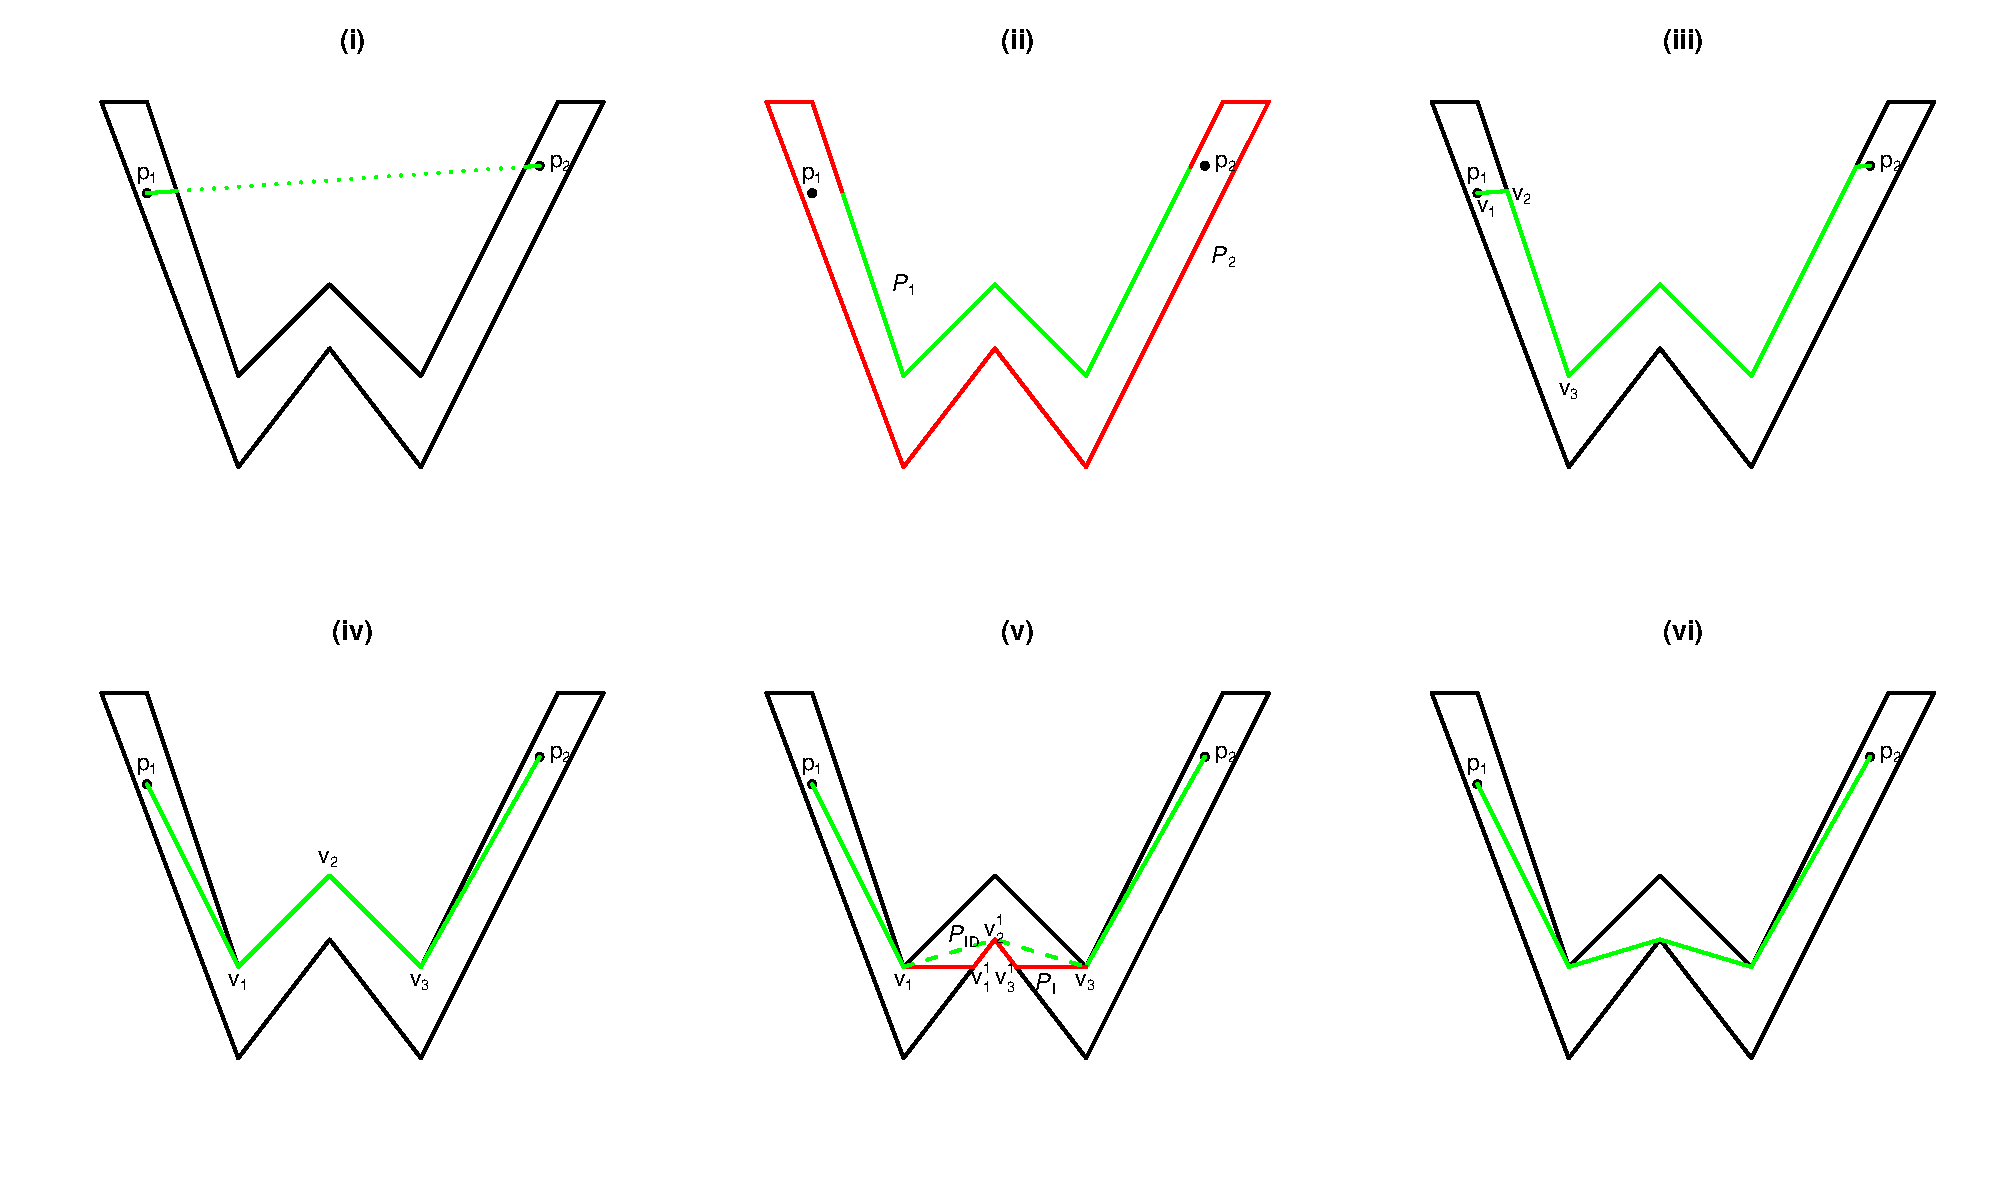
\includegraphics[angle=90, height=\textheight,trim=0in 0.5in 0in 0.25in]{figs/wdia.pdf} \\
%\label{wdia}
%%\caption{The green lines in ($i$) to ($vi$) show the steps forming the shortest path as the algorithm progresses from initial state to final, shortest path (bottom right). See Appendix B for more details.}
%% generated by figs/distanceexplanation.R
%\end{figure}
%



Of course, if there is a direct path between $p_1$ and $p_2$ then the Euclidean distance between the points can be used and the above algorithm is not run.

Although the authors were not able to prove theoretically that the algorithm will always converge to the shortest path, it is clear at least the the algorithm will always converge (since this only requires that there be no change in the path for two consecutive iterations). Extensive simulations showed that the algorithm gave sensible results.


\subsection*{Speed improvement via partial path calculation}

It is often the case that the points for which distances are required form a grid (for example, the initial MDS grid, or prediction points). This grid setup can be exploited since there are many sets of paths that are rather similar. These paths may perhaps only differ in their final vertex. When this is the case much computational time is wasted calculating similar paths, we can exploit this problem to increase the speed of the path calculation.

By appending the points between which the within-area distance is required to either end of one of a series of pre-calculated base paths, then optimising this new path using the DELETE and ALTER steps as before,  the computational time taken to find the paths is reduced. Using base paths removes the expensive calculation in the middle of the path, where the bulk of the interactions with the boundary take place.

The algorithm is as follows, with notation and routines (INIT, DELETE, ALTER and ITER) identical to those above:
\begin{enumerate}
 \item Begin by creating a sparse grid of within the simple polygon $\Gamma$ and calculate the ($M$, say) non-Euclidean within-area paths between all pairs of points in the grid, as above. Store these paths as $\mathcal{P}_1,\ldots, \mathcal{P}_M$.
\item For each unique pairing of $p_i$ and $p_j$ in the full data set, calculate the path using one of the following:
\begin{enumerate}
\item Find a $\mathcal{P}_k$ such that the path between $p_i$ and one end of $\mathcal{P}_k$ and $p_j$ and the other end of $\mathcal{P}_k$ is Euclidean within $\Gamma$. Join $p_i$ and $p_j$ onto the appropriate ends of $\mathcal{P}_k$ and alternate between DELETE and ALTER steps until convergence.
\item If no $\mathcal{P}_k$ can be found calculate the path between $p_i$ and $p_j$ as above. 
\end{enumerate}
\end{enumerate}

Note that those paths between points in the sparse grid which are Euclidean are not stored since it is always at least as expensive to store, add to and optimise those paths then calculating them from scratch. If the required path is Euclidean anyway, then retrieving a Euclidean path, adding in $p_i$ and $p_j$, and then iterating over ALTER and DELETE steps to make it both the shortest and a Euclidean path will take longer than just creating a Euclidean path to begin with. If the path between $p_i$ and $p_j$ is non-Euclidean then the non-Euclidean part of the path must lie outside $\mathcal{P}_k$ (by definition, if $\mathcal{P}_k$ were Euclidean) and therefore will take the same number of operations to find the boundary crossing points and calculate the shortest path around the feature locally as it will to calculating the whole path from scratch.

This speed-up reduced the time to fit MDSDS to the peninsulae domain above (without MDS dimension selection) from 84 seconds to 18 seconds on a MacBook Air (2,1) with a 1.86GHz Intel Core 2 Duo processor.

This algorithm could be further improved by finding optimal starting grids. Adapting the methods described in L{\o}land and H{\o}st (2003) to approximate the distances using a triangulation, could increase performance (although perhaps at the price of accuracy).

\begin{thebibliography}{99}

\bibitem{} Augustin, N.H., Musio, M., von Wilpert, K., Kublin, E., Wood, S.N. and Schumacher, M. (2009). 
Modeling spatiotemporal forest health monitoring data. \textit{Journal of the American Statistical Association} \textbf{104}(487), 899--911.

\bibitem{} Bernstein, M., de Silva, V., Langford, J.C., and Tenenbaum, J.B. (2000). Graph approximations to geodesics on embedded manifolds. Technical report.

\bibitem{} Boisvert, J.B., Manchuk,  J.G. and Deutsch, C.V. (2009). Kriging in the presence of locally varying anisotropy using non-{E}uclidean distances. \textit{Mathematical Geosciences} \textbf{41}, 585--601.

\bibitem{} Chatfield, C. and Collins, A.J. (1980). \textit{Introduction to multivariate analysis}. CRC Press.

\bibitem{} Craven, P. and Wahba, G. (1979), Smoothing noisy data with spline functions. \textit{Numerische Mathematik} \textbf{31}, 377--403.

\bibitem{} Curriero, F. (2006). On the use of non-{E}uclidean distance measures in geostatistics. \textit{Mathematical Geology} \textbf{38}(8), 907--926.

\bibitem{} Diggle, P.J. and Ribeiro, P.J. (2007). \textit{Model-based Geostatistics}. Springer.

\bibitem{} 	Driscoll, T.A. and Trefethen, L.N. (2002). \textit{Schwarz-Christoffel Mapping}. Cambridge University Press.

\bibitem{} Floyd, R.W. (1962). Algorithm 97: Shortest path. \textit{Communications of the ACM} \textbf{5}(6), 345.

\bibitem{} Gentleman, R., Ding, B., Dudoit, S., and Ibrahim, J. (2005). Distance measures in DNA microarray data analysis. In R. Gentleman, V. Carey, W. Huber, R. Irizarry, and S. Dudoit (Eds.), \textit{Bioinformatics and Computational Biology Solutions Using R and Bioconductor}, pp. 189--208. Springer.

\bibitem{} Girosi, F., Jones, M. and Poggio, T. (1995). Regularization theory and neural networks architectures. \textit{Neural computation}, \textbf{7}, 219-269.

\bibitem{} Gower, J.C. (1966). Some distance properties of latent root and vector methods used in multivariate analysis. \textit{Biometrika}, \textbf{53}(3 and 4), 325--338.

\bibitem{} Gower, J. C. (1968). Adding a point to vector diagrams in multivariate analysis. \textit{Biometrika}, \textbf{55}(3), 582--585.

\bibitem{} Hart, P. E., Nilsson, N. J. and Raphael, B. (1968). A Formal Basis for the Heuristic Determination of Minimum Cost Paths. \textit{IEEE Transactions on Systems Science and Cybernetics SSC4} \textbf{4}(2), 100--107.

\bibitem{} Hastie, T. and Tibshirani, R. (1990). \textit{Generalized Additive Models}. Chapman \& Hall.

\bibitem{} Hastie, T., Tibshirani, R. and Friedman, J. (2001). \textit{Elements of Statistical Learning}. Springer.

\bibitem{ } Hedley, S.L. and Buckland, S.T. (2004) Spatial Models for Line Transect Sampling. \textit{Journal of Agricultural, Biological, and Environmental Statistics} \textbf{9}(2), 181--199.

\bibitem{} L{\o}land, A. and H{\o}st, G. (2003). Spatial covariance modelling in a complex coastal domain by multidimensional scaling. \textit{Environmetrics} \textbf{14}(3), 307--321.

\bibitem{} Jensen, O.P., Christman, M.C. and Miller, T.J. (2006). Landscape-based geostatistics: a case study of the distribution of blue crab in {C}hesapeake {B}ay. \textit{Environmetrics} \textbf{17}(6), 605--621.

\bibitem{} Mahalanobis, P.C. (1936). On the generalised distance in statistics. \textit{Proceedings of the National Institute of Sciences of India} \textbf{2}(1), 49--55.

\bibitem{} Marra, G. and Radice, R. (2010). Penalised regression splines: theory and application to medical research. \textit{Statistical Methods in Medical Research}, 19, 107--125.

\bibitem{} Miller, D.L. (2011) \textit{On smooth models for complex domains and distances}. PhD thesis, University of Bath.

\bibitem{} Oh, M-S and Raftery, A.E. (2001). Bayesian multidimensional scaling and choice of dimension. \textit{Journal of the American Statistical Association}, \textbf{96}(455), 1031--1044.

\bibitem{} Ramsay, T. (2002). Spline smoothing over difficult regions. \textit{Journal of the Royal Statistical Society: Series B} \textbf{64}(2), 307--19.

\bibitem{} Ruppert, D., Wand, M.P. and Carroll, R.J. (2003). \textit{Semiparametric Regression}. Cambridge University Press.

\bibitem{} Ruppert, D., Wand, M.P. and Carroll, R.J. (2009). Semiparametric regression during 2003--2007. \textit{Electronic Journal of Statistics}, \textbf{3}, 1193--1256.

\bibitem{} Scott-Hayward, L.A.S., Mackenzie, M.L., Donovan, C.R., Walker, C.G. and Ashe, E. (under review) Complex Region Spatial Smoother (CReSS). \textit{A Journal}.

\bibitem{} Shabenberger, O. and Gotway, C.A. (2005). \textit{Statistical methods for spatial data analysis}. CRC Press.

\bibitem{} de Silva, V. and Tenenbaum, J.B. (2004). Sparse multidimensional scaling using landmark points. Tech report, Stanford University.

\bibitem{} Venables, W.N. and Ripley, B.D. (2002). \textit{Modern applied statistics with S}. Springer.

\bibitem{} Vretblad, A. (2003). \textit{Fourier Analysis and Its Applications}. Springer.

\bibitem{} Wang, H. and Ranalli, M.G. (2007). Low-rank smoothing splines on complicated domains. \textit{Biometrics} \textbf{63}(1), 209--217

\bibitem{} Williams, R., Hedley, S.L., Branch, T.A. and Bravington, M.V., Zerbini, A.N. and Findlay, K.P. (2011). Chilean Blue Whales as a Case Study to Illustrate Methods to Estimate Abundance and Evaluate Conservation Status of Rare Species. \textit{Conservation Biology} \textbf{25}(3), 526--535.

\bibitem{} Wood, S.N. (2003). Thin plate regression splines. \textit{Journal of the Royal Statistical Society: Series B}, \textbf{65}(1) 95--114.

\bibitem{} Wood, S.N. (2006). \textit{Generalized Additive Models: An Introduction with R}. Chapman \& Hall.

\bibitem{} Wood, S.N. (2011). Fast stable restricted maximum likelihood and marginal likelihood estimation of semiparametric generalized linear models. \textit{Journal of the Royal Statistical Society: Series B}, \textbf{73}(1), 3--36.

\bibitem{} Wood, S.N., Bravington, M.V. and Hedley, S.L. (2008). Soap film smoothing. \textit{Journal of the Royal Statistical Society Series B} \textbf{70}(5), 931--55.

\end{thebibliography}


\label{lastpage}

\end{document}

